Particle A is around \unit[24]{$\mu m$} long so it has a $\lambda$ of close to 8 and the closest match for the asymetry is $\epsilon = 0.02$. To see how good of a fit these parameters actually are we can look at the goodness of fit fo the asymetry in figure \ref{fig:asymVariation}, the matched orbit for stretch 1 of measurement 1 figure \ref{fig:orbitVariation} and the starting position (initial $\psi$) for that orbit in figure \ref{fig:initVariation}.  

\begin{figure}[H]
\begin{center}
\includegraphics[width=0.7\textwidth]{figures/results/particleA/A_assymVariation.pdf}
\end{center}
\caption{We see how the difference between the theoretical $n_z$ and all the measured  $\widetilde{n_z}$ for all measurements of particle A for different asymmetries $\epsilon$. For each asymmetry we find the orbit and the initial $\psi$ with the smallest distance for each stretch.}
\label{fig:asymVariation}
\end{figure}

\begin{figure}[H]
\begin{center}
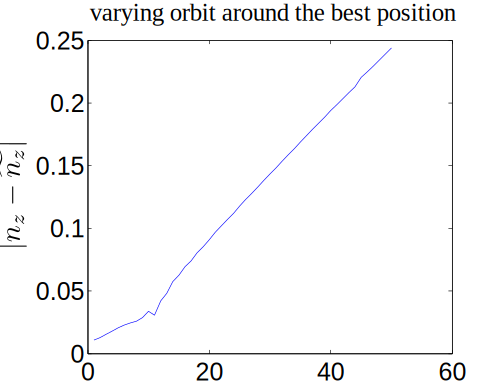
\includegraphics[width=0.7\textwidth]{figures/results/particleA/A_orbitVariation.pdf}
\end{center}
\caption{The difference between the theoretical $n_z$ and the measured $\widetilde{n_z}$ for the first stretch of the first measurement for particle A (seen in figure \ref{fig:particleA1})with the best asymmetry for different orbits. .}
\label{fig:orbitVariation}
\end{figure}


\begin{figure}[H]
\begin{center}
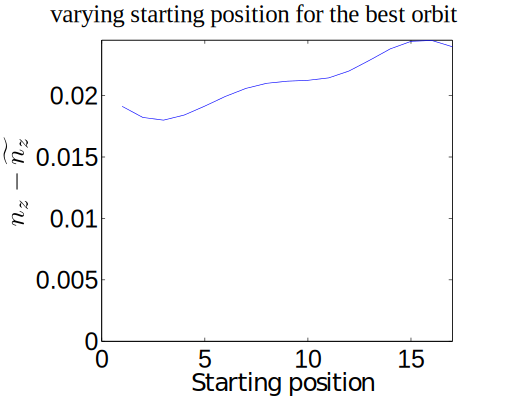
\includegraphics[width=0.7\textwidth]{figures/results/particleA/A_posVariation.pdf}
\end{center}
\caption{The difference between the theoretical $n_z$ and the measured $\widetilde{n_z}$ for the first stretch of the first measurement for particle A. The best orbit and best asymmetry are chosen, but different initial conditions are tested. }
\label{fig:initVariation}
\end{figure}


Looking at figure \ref{fig:particleAOrbitFit} and we can see that particle A is in a quasi-periodic circular orbit during measurement 1 (the lines indicating A B and C). We can see in figure \ref{fig:particleAreversegood}] has an almost perfectly matching reversal which means there was no significant amount of noise or sinking present during this measurement. After being shifted by  the optical tweezer we can see in figure \ref{fig:particleA2} that it also followed a periodic orbit during measurement 2. 



\begin{figure}[H]
\begin{center}
\includegraphics[width=0.7\textwidth]{figures/results/particleA/October11Particle2_Orbits_Added.pdf}
\end{center}
\caption{Gray lines are the phase map for $\lambda = 8$ and $\epsilon = 0.02$. The measured $\lambda$ was $8.2 \pm 0.1$. The orbits of the best fit theoretical fits to measurements are highlighted stretch by stretch. Most measured orbits for this particle were rather constant, but the winding numbers are within 50\% of the estimates but both are too low, suggesting that the $\epsilon$ might be too low.}
\label{fig:particleAOrbitFit}
\end{figure}

%lambda = [8.27, 8.027, 8.1205, 8.2401, 8.2401, 8.1637]

\subsection{Measurement 1}
\begin{figure}[H]
\begin{center}
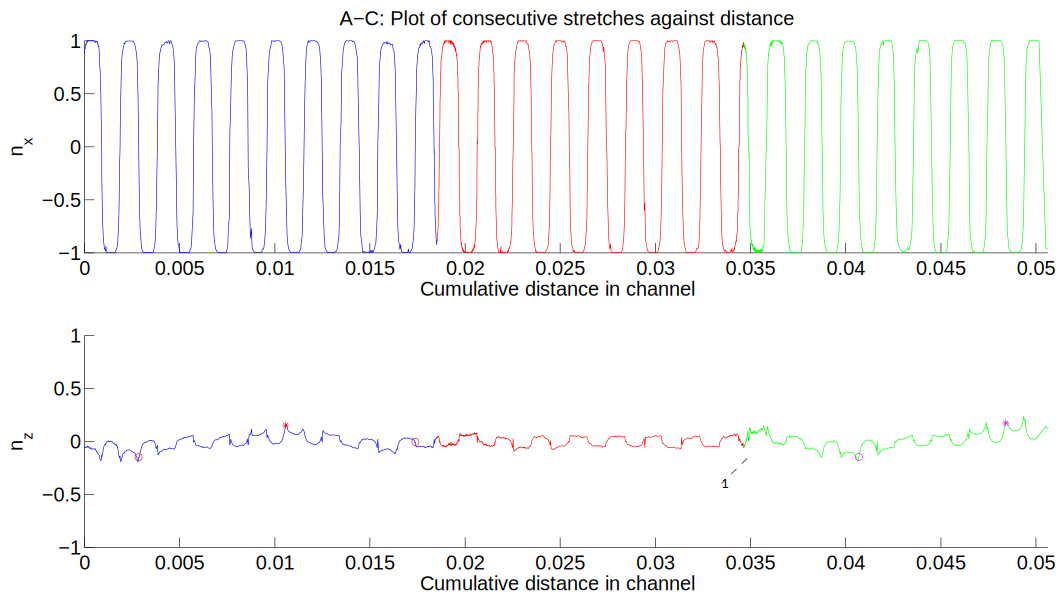
\includegraphics[width=0.7\textwidth]{figures/results/particleA/October_11_Particle_2_run_2_winding.pdf}
\end{center}
\caption{The estimate $n_x$ and $n_z$ components of the particle. Despite being very close to a centre orbit there is very little quasi-periodic behaviour. The very flattened peaks compared to a low $n_z$ orbit in \ref{fig:orbitparams} are a result of the width compensation discussed in section \ref{sec:width_compensation}. This particle started $x_0 = 9.8 mm, z_0 = 8.9924 \mu m$ and $D \approx 90\mu$m.}
\label{fig:particleA1}
\end{figure}

\begin{figure}[H]
\begin{center}
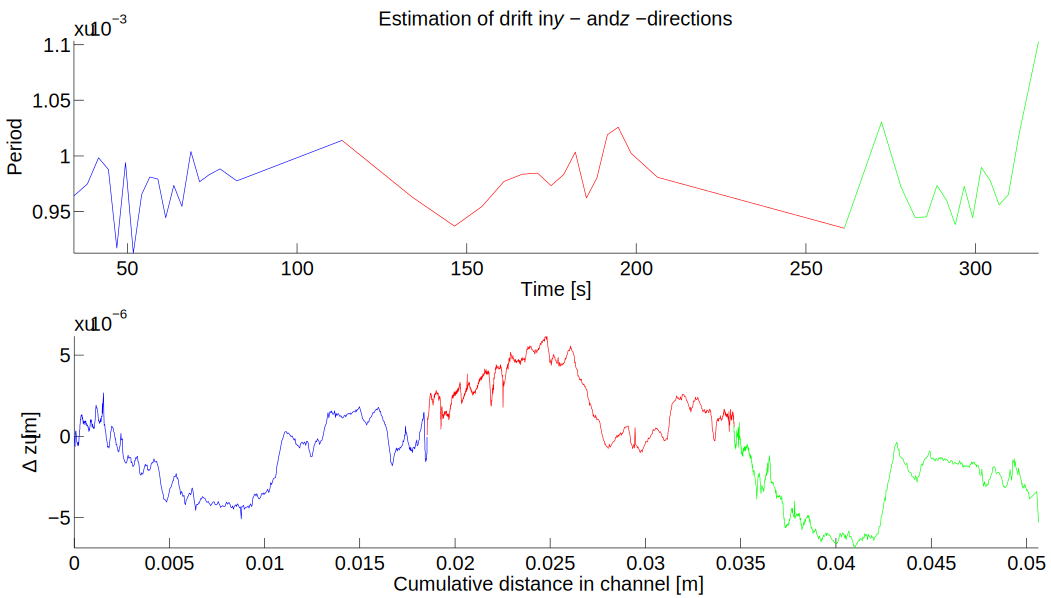
\includegraphics[width=0.7\textwidth]{figures/results/particleA/October_11_Particle_2_run_2_B.pdf}
\end{center}
\caption{Estimation of the sinking of the particle and the z position in the channel. The period here refers to the distance between two successive zeros for $n_x$ relative to the first. There is no clear trend to higher or lower values which suggests that there is little sinking/floating. The drift in the z coordinate is very small relative to the movements in the x direction. Z-direction movements are on the order of $10\mu m$ compared to the x direction which is on the order of $2\cdot 10^4 \mu m$}
\label{fig:particleAsink}
\end{figure}

\begin{figure}[H]
\begin{center}
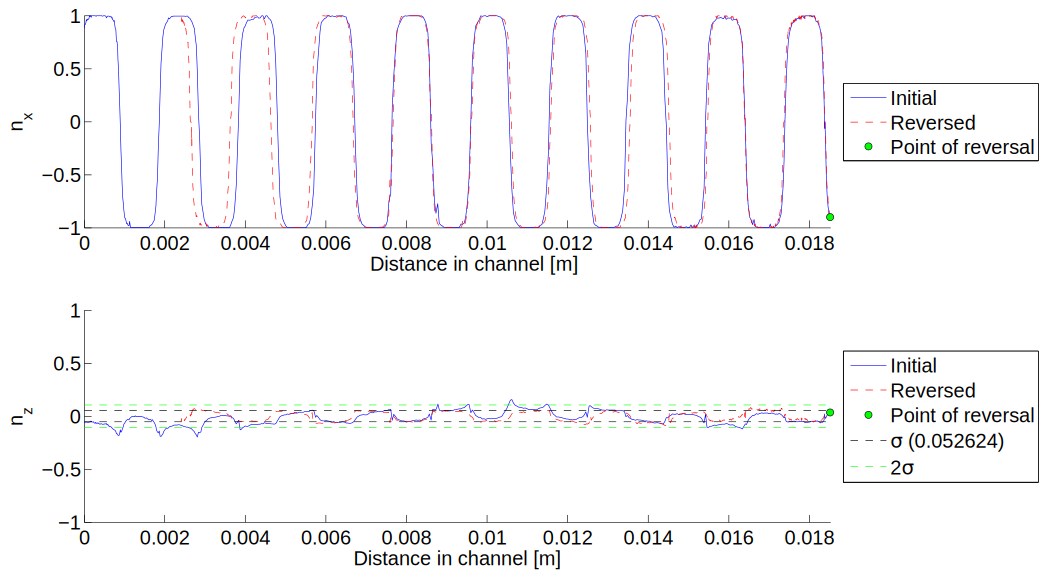
\includegraphics[width=0.7\textwidth]{figures/results/particleA/October_11_Particle_2_run_2_C01.pdf}
\end{center}
\caption{Shows $n_x$ and $n_x$ first and second stretches from Measurement 1, seen in figure \ref{fig:particleA1} but against the actual position in the channel as opposed to comulative distance. There is an almost perfect match along the entire channel for $n_x$ and only small disagreement for $n_z$. The dashed lines indicate the error margins for detecting $n_z=0$. This figure is the same as can been seen in Laas\cite{alexanderThesis} figure 6.21}
\label{fig:particleAreversegood}
\end{figure}

\begin{figure}[H]
\begin{center}
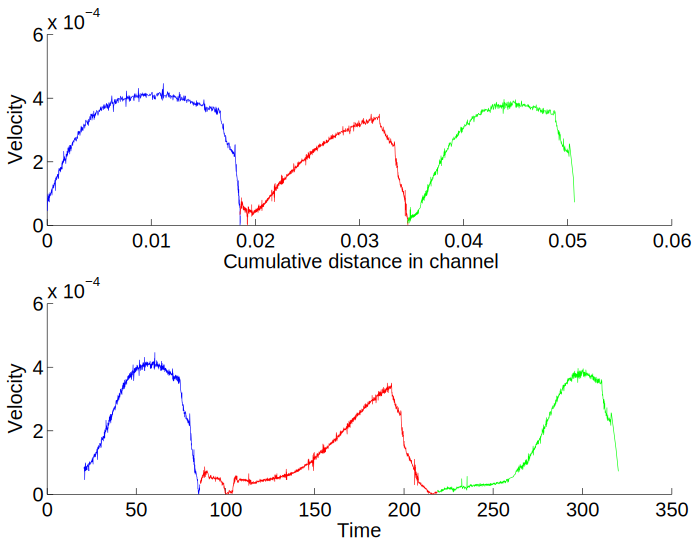
\includegraphics[width=0.7\textwidth]{figures/results/particleA/October_11_Particle_2_run_2_D.pdf}
\end{center}
\caption{The speed (note not the velocity) of the particle against distance as well as time. The most distinct difference is in the time plot where we see in the first reversal there is a "double dip". This only and always occurs at the reversal at the far end from the pump. There is also noticeably different acceleration behaviour that is consistently different across all measurements.}
\label{fig:particleAspeed}
\end{figure}

\subsection{Measurement 2}

\begin{figure}[H]
\begin{center}
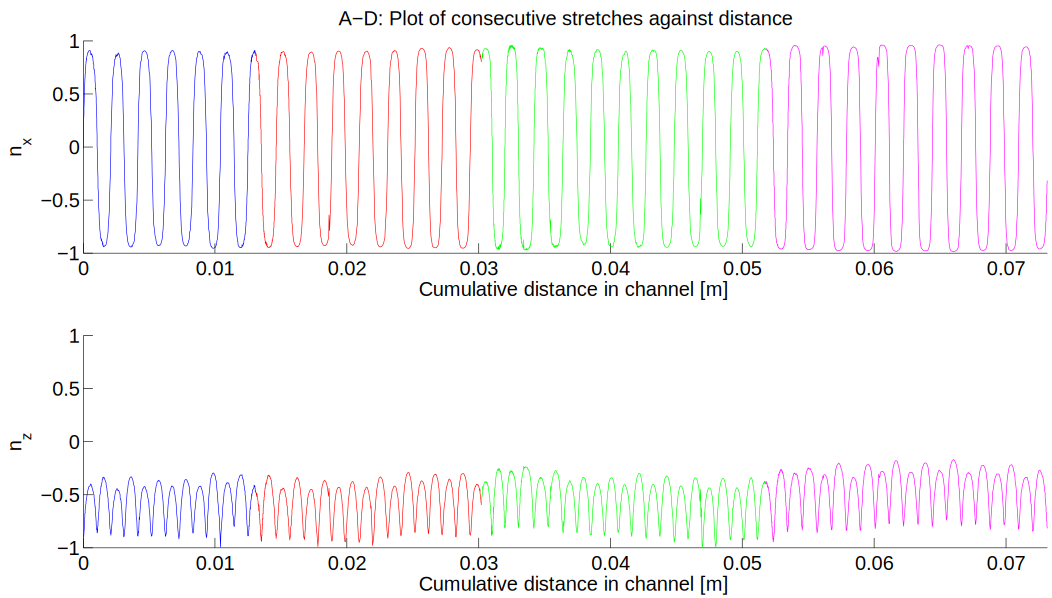
\includegraphics[width=0.7\textwidth]{figures/results/particleA/October_11_Particle_2_run_3_A.pdf}
\end{center}
\caption{A tracked particle with a large $n_z$ component with a very consistent periodic behaviour. 
$ x_0 = 26.0 mm, z_0 = 275\mu m, D\approx 105\mu$ m.}
\label{fig:particleA2}
\end{figure}

\subsection{Measurement 3}
\begin{figure}[H]
\begin{center}
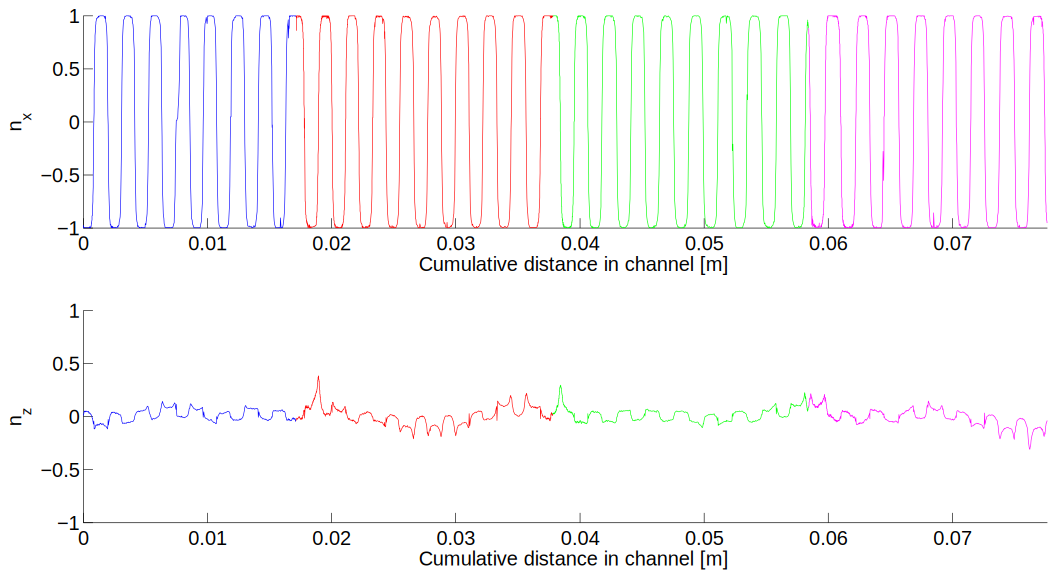
\includegraphics[width=0.7\textwidth]{figures/results/particleA/October_11_Particle_2_run_6_A.pdf}
\end{center}
\caption{The peaks that occur after each reversal are not the cause of a tracking error but can be seen clearly in the films. The cause of such a sudden peak and then reverting back to another orbit is not known and we have no good theoretical explanation for it. We begin to break around (3) which is also where there is a change in the orbit. The particle starts at $ x_0 = 12.3 mm, z_0 = 160 \mu m, D \approx 100\mu$m.}
\label{fig:particleA3}
\end{figure}



\subsection{Measurement 4}
\begin{figure}[H]
\begin{center}
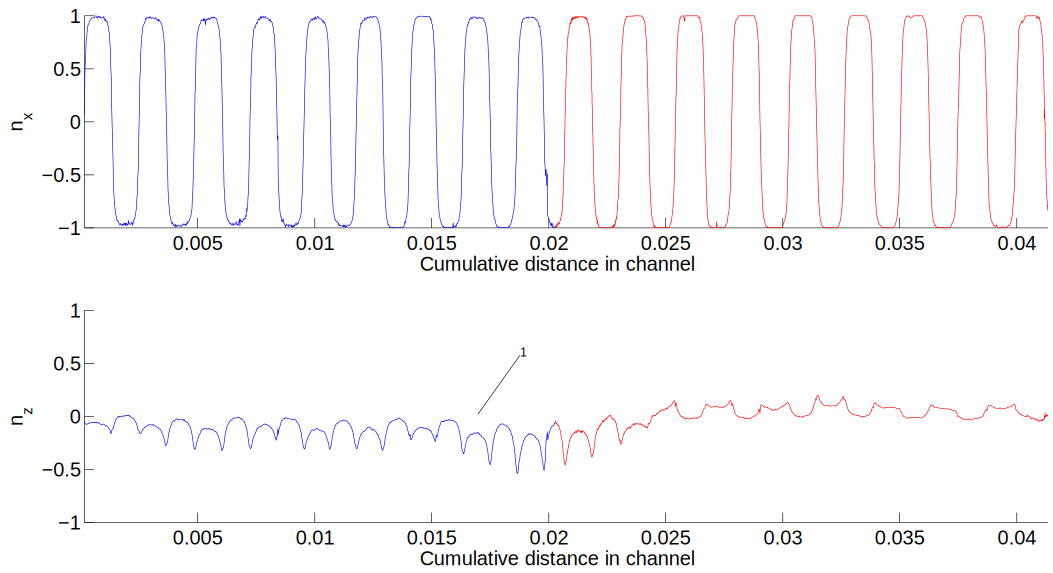
\includegraphics[width=0.8\textwidth]{figures/results/particleA/October_11_Particle_2_run_1_A.pdf}
\end{center}
\caption{The flow is reversed when the particle is at (1) and and we can see that the peaks are larger than what we would expect from the rest of the stretch. Started at $x_0 = 8.7 mm, z_0 = 16\mu m, D \approx 95\mu$m.}
\label{fig:particleA4}
\end{figure}

\subsection{Measurement 5}
\begin{figure}[H]
\centering
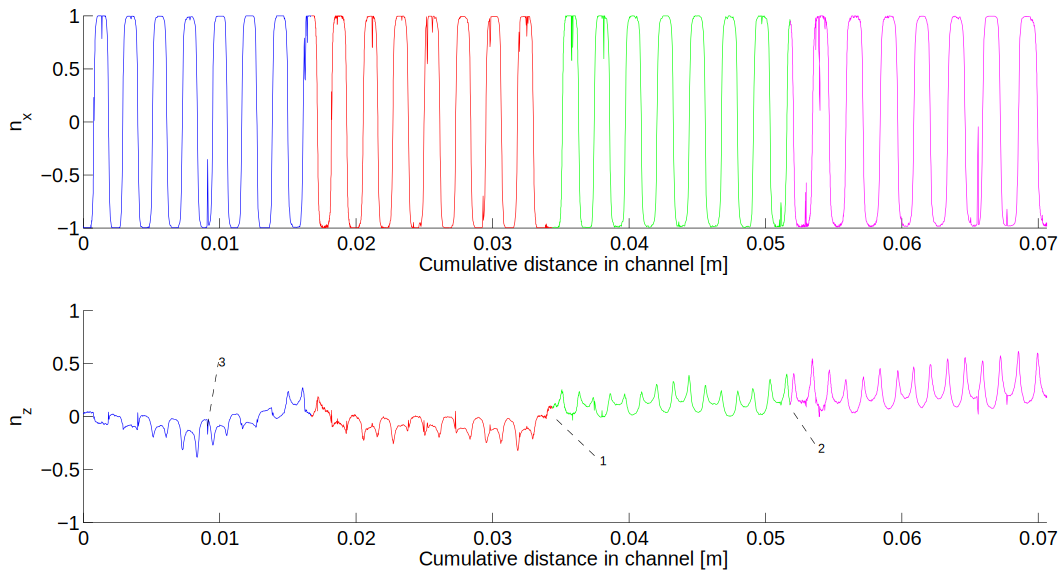
\includegraphics[width=0.8\textwidth]{figures/results/particleA/October_11_Particle_2_run_4_A.pdf}
\caption{$x_0 = 10.7 mm, z_0 = 240 \mu m, D \approx 60\mu m$.
1: Very bad reversal. Note that this very bad reversal occurs at the "pump side" of the channel. 
 2: A slight change in orbit, but it is still in the same region on the SOS.
 3: Data that haven't been cleaned.}
\label{fig:particleA5}
\end{figure}

 
 \begin{figure}[H]
 \centering
 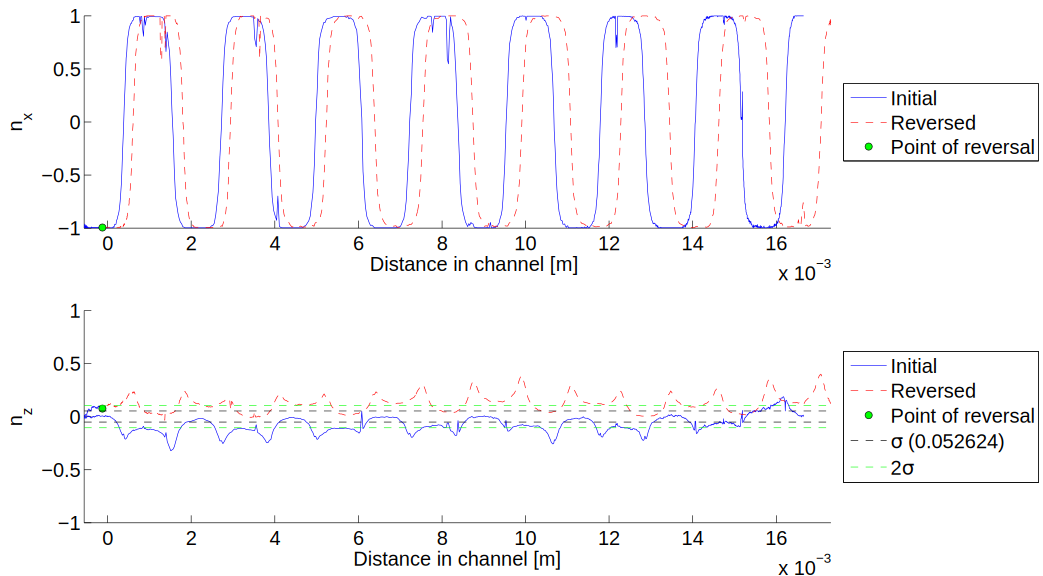
\includegraphics[width=0.8\textwidth]{figures/results/particleA/October_11_Particle_2_run_4_C02.pdf}
 \caption{$n_x$ and $n_z$ from figure \ref{fig:particleA5} for the second and third stretch plotted against actual distance instead of commutative distance. The reversal occurs at the left and although there is some moderate agreement in $n_x$ the match in $n_z$ is non existant from the very start.}
 \label{fig:particleABadReversal}
 \end{figure}